\section{Recoil separators at radioactive ion beam facilities}

\subsection{FMA}
The Fragment Mass Analyzer at Argonne National Laboratory~\cite{Da92} was designed for study of high-spin states following heavy-ion fusion.  Like mass separators at Rochester and Legnaro, the FMA has a series of electric, magnetic and electric dipoles.   At $\Delta$V=425~kV and each of length 1.4~m, the two electrostatic dipoles have proxy figure of merit 1260~kV$\cdot$m.  Design acceptances were $\pm$20\% in energy and 8~msr solid angle ($\pm2.3^{\circ}$ in the non-dispersive plane, $\pm2.8^{\circ}$ in the dispersive plane \cite{dav12}), with M/q resolving power of 340.

Although the FMA was not designed to study radiative capture reactions, it was used to successfully study the \pgamma{18}{O}{19}{F}, and  \pgamma{18}{F}{19}{Ne} reaction \cite{reh97} (achieving an upper limit on a resonance at \EcmM{0.66}). No further radiative capture reactions have been studied at the facility since this time. It shows however, that recoil separators of this type {\em can} in principle be used for radiative capture, a fact that has implications for future separators of the same EME configuration, such as EMMA at TRIUMF-ISAC. 


\subsection{ARES - Louvain-la-Neuve}

The Astrophysics Recoil Separator (ARES) was the first recoil separator at an ISOL radioactive ion beam facility designed for measurements of \reac{p}{\gamma} reactions in inverse kinematics. It was coupled to the CYCLONE44 cyclotron at the Cyclotron Research Center in Louvain-la-Neuve (Belgium). The cyclotron was dedicated to the acceleration of radioactive ion beams (available in sufficient intensity: \nuc{13}{N} and \nuc{19}{Ne}) in the (0.2 -- 0.8)$\cdot A$ MeV energy range. Compared to electrostatic or linear accelerator facilities CYCLONE44 produces beam with relatively large energy spread ($\frac{\Delta{}E}{E} \approx 1\%$) and emittance ($28\pi \unit{mm\,mrad}$ (horizontal) and $16\pi \unit{mm\,mrad}$ (vertical)), which complicate significantly experiments with recoil separators.
\begin{figure*}
\begin{center}
\resizebox{1.5\columnwidth}{!}{
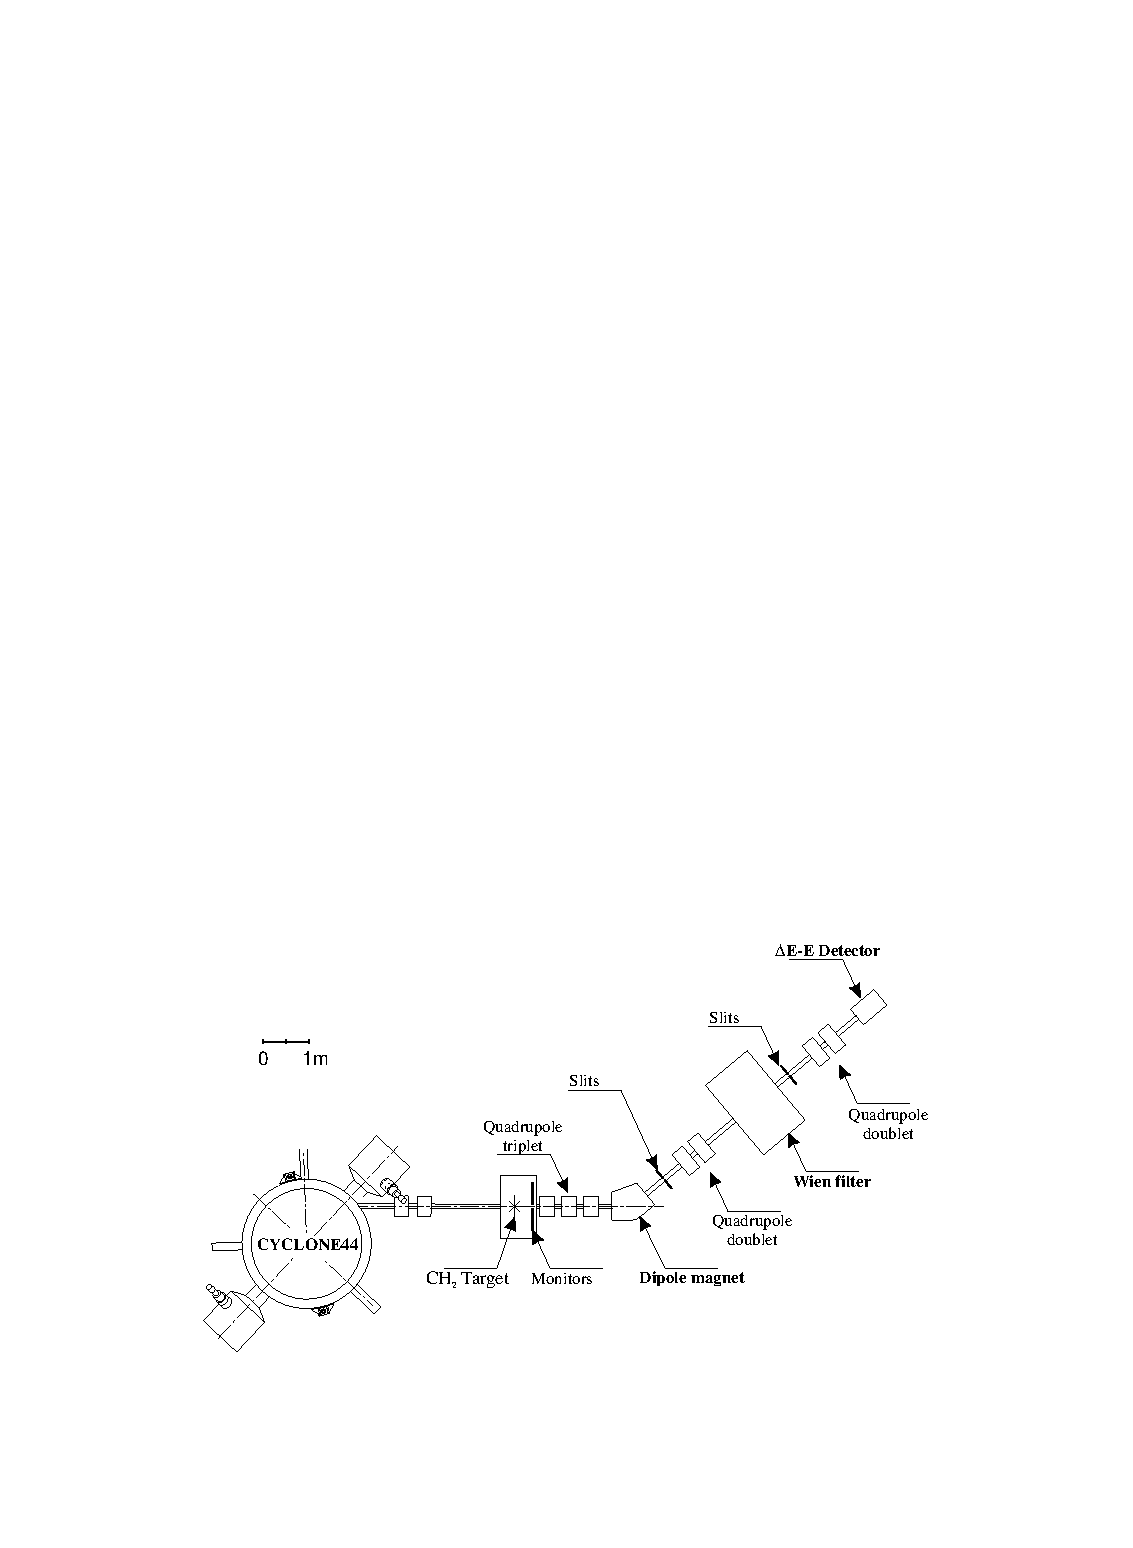
\includegraphics{Couder03_Fig1_ARES}
}
%\vspace{5cm}       % Give the correct figure height in cm
\caption{Schematic view of the ARES separator. Taken from \cite{coud03}.}
\label{fig:ares}
\end{center}
\end{figure*}
Additionally, ARES did not have a gas target available but operated with a plastic foil (CH$_2$) hydrogen target, see Fig. \ref{fig:ares}, thereby reducing resonant yield, and producing additional energy and angle straggling to cope with. The rest of the setup followed the NABONA approach of first using a magnetic dipole to select a charge state to transport and then a crossed field (Wien-) filter to suppress the beam ions of the selected charge state. For recoil detection a $\Delta{}E$-$E$ system combining energy loss measurement in an ionization chamber and rest energy detection in a silicon (PIPS) detector was used \cite{coud03}. Due to the large emittance of the beam direct measurements of the transport efficiency of the separator alone (and thereby deduction of an acceptance) was not possible. Instead, a measurement of the nuclear reaction \nuc{19}{F}\reac{p}{\gamma}\nuc{20}{Ne} was performed in inverse kinematics, and the result compared to simulation and literature data. For this reaction, a selected charge state of the \nuc{20}{Ne} recoils was transported with approximately 11\% transmission efficiency (simulation and experiment in agreement). The rejection factor of the separator proved to be of the order of only $10^{-7}$ resulting from the poor ion beam quality as well as the use of a solid foil target \cite{angu01,coud05}. Nevertheless, the ARES collaboration attempted a measurement of the \nuc{19}{Ne}\reac{p}{\gamma}\nuc{20}{Na} reaction to populate a resonant state at 448 keV having of the order of $10^8 ~\unit{s^{-1}}$ \nuc{19}{Ne} ion beam available. No recoils were detected and an upper limit on the resonance strength of $\omega\gamma = 15.2 \unit{meV}$ established. This limit represents the sensitivity of the separator as defined by the efficiency and primary beam suppression. No further experiments at ARES were performed.

\subsection{DRS - Holifield Radioactive Ion Beam Facility}

The Daresbury Recoil Separator (DRS) was initially designed for use in the UK for the measurement of fusion evaporation reactions in nuclear structure research. With the closure of its accelerator facility, the separator became available for nuclear astrophysics research and was relocated to the newly dedicated Holifield Radioactive Ion Beam Facility (HRIBF) at Oak Ridge National Laboratory (ORNL) \cite{smit98}. It follows in principle the Caltech approach of using a velocity filter (crossed fields) to separate recoils from beam followed by a magnetic dipole ($50^\circ$) to separate charge states. It featured the improvement that two velocity filters were installed in sequence with an additional focus and selection slits in between them, as shown in Fig.\ \ref{fig:drs}.
\begin{figure*}
\begin{center}
\resizebox{1.5\columnwidth}{!}{
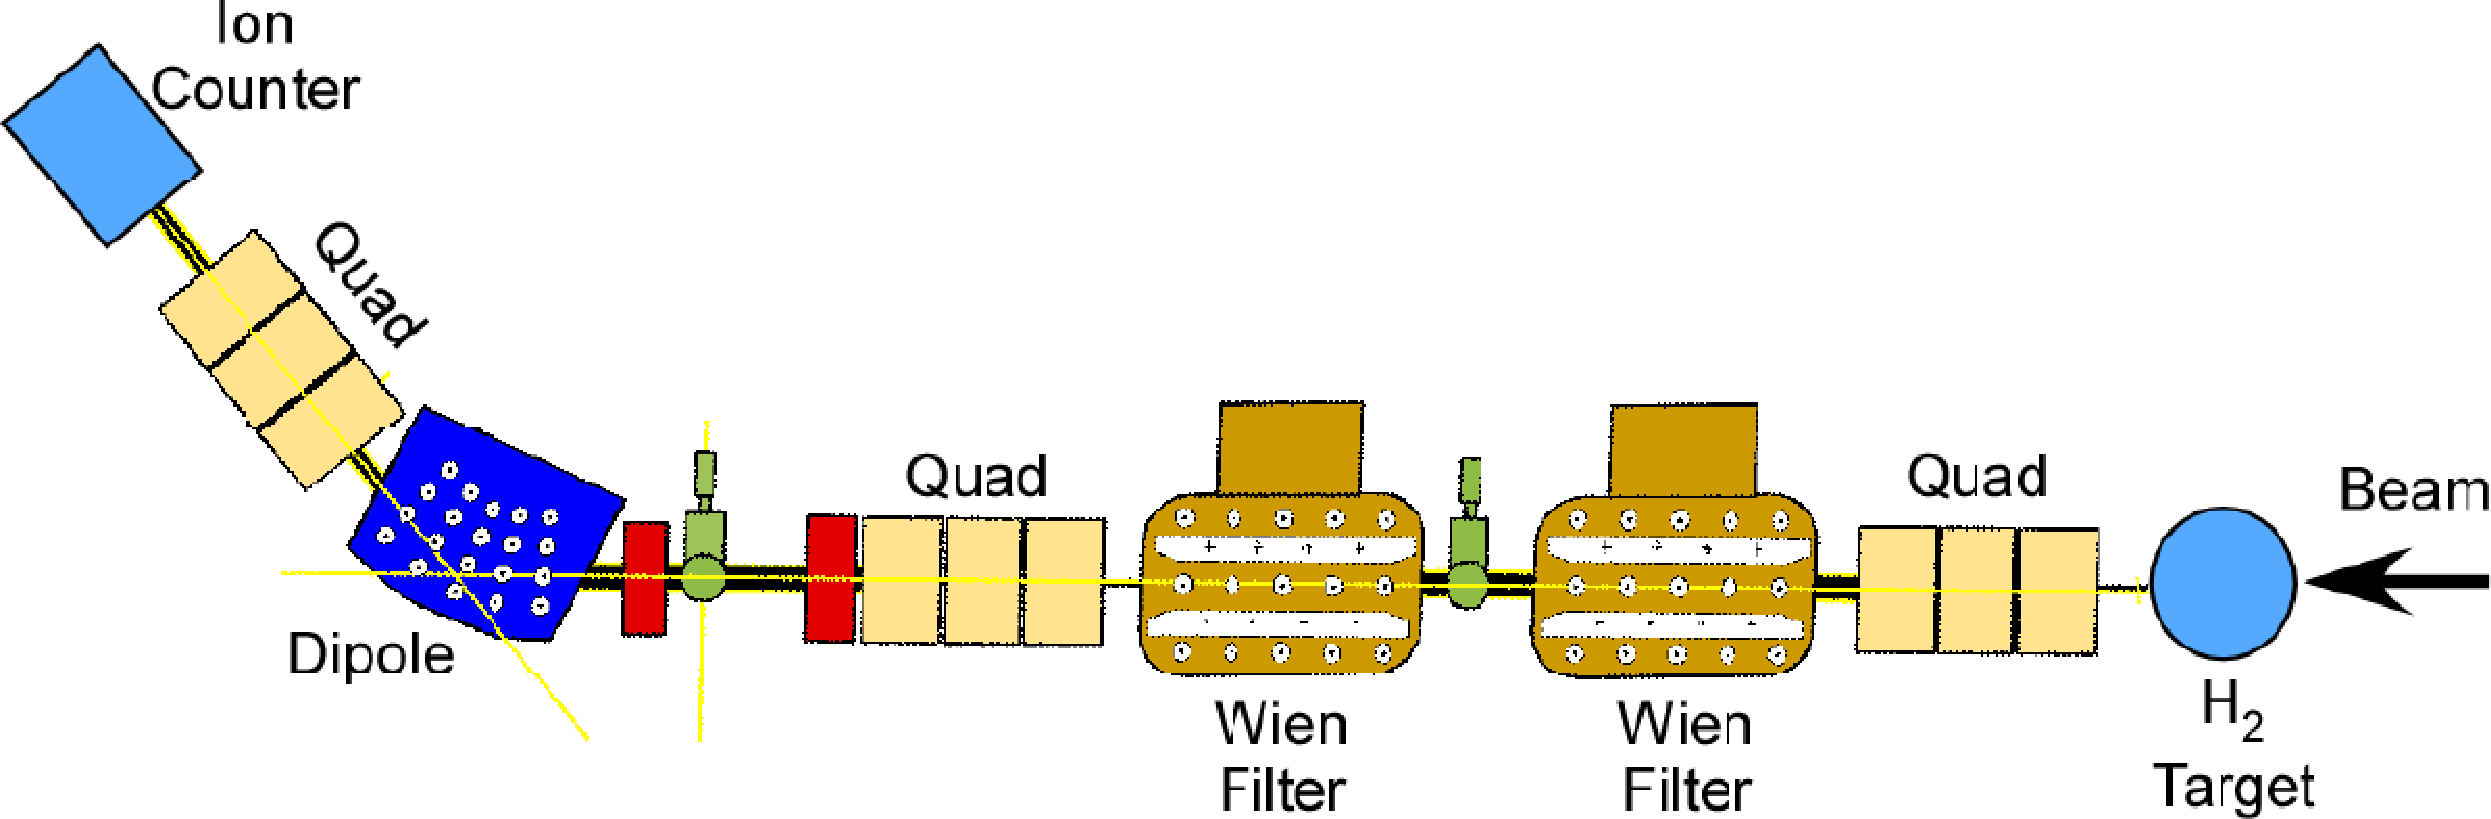
\includegraphics{Bardayan09_Fig1_DRS}
}
%\vspace{5cm}       % Give the correct figure height in cm
\caption{Schematic view of the DRS separator. Dispersive elements are a pair of Wien filters followed by a 50-degree magnetic dipole.   With maximum design voltage $\Delta$V=600~kV and each of length 1.28~m, the two Wien filters have a proxy figure of merit 1536~kV$\cdot$m.
Design acceptances were 2$\times$45~mrad in horizontal and vertical angles, $\pm$2\% in velocity and  $\pm$1.2\% in M/q, with resolving power 300 in M/q.Taken from \cite{bard09}.}
\label{fig:drs}
\end{center}
\end{figure*}
The HRIBF uses a light ion cyclotron to drive an on-line radioactive ion source which injects negative ions into the vertical folded tandem accelerator with a maximum terminal voltage of 25 MV. For nuclear astrophysics research the facility focused on the production of radioactive fluorine isotopes relevant to the hot and explosive CNO cycles. Measurement of radiative capture in this mass regime however required running the Tandem close to the lower voltage limits sacrificing transmission efficiency. For these measurements the DRS was coupled with a windowless Hydrogen gas target capable of maintaining 5.5 Torr pressure over 15 cm target length. The acceptance of the separator was only limited in these experiments by the diameter of the gas flow limiting apertures. These were tailored to accept the specific reaction recoils pursued. In the final focal plane of the separator a $\Delta{}E-E$ ionization chamber (IC) provided nuclear charge (Z) identification. Additionally, a position sensitive MCP detector was available to position in front of the IC to map the recoil hit positions. Ion beam suppression factors of order $10^9 - 10^{11}$ were achieved, varying with beam energies and conditions. The DRS was tested with proton capture on stable \nuc{24}{Mg}, \nuc{17}{O} and \nuc{12}{C} and used for measurement of the radioactive beam reactions \nuc{1}{H}(\nuc{17}{F},$\gamma$)\nuc{18}{Ne} and \nuc{1}{H}(\nuc{7}{Be},$\gamma$)\nuc{8}{B}. 


\subsection{DRAGON - TRIUMF-ISAC}
The DRAGON Facility (Detector of Recoils And Gammas Of Nuclear reactions) was designed to provide a recoil separator to study radiative capture reactions, both on protons and alpha particles, using post-accelerated radioactive ion beams at the ISAC facility \cite{hut03a,hut03,eng05}. The ISAC facility \cite{ball11} provides ISOL beams using a 75$\mu$A, 500 MeV proton beam from the TRIUMF sector-focusing cyclotron. These are reaccelerated through a 35 MHz radio-frequency quadrupole with $A/q\leq30$, and a 105 MHz variable energy drift-tube-linac with $3\leq A/q\leq6$, between energies of 0.15$A$ MeV and 1.5$A$ MeV \cite{lax02}.  This energy regime, particularly the lower end, is well-suited to performing radiative capture reactions of the type occurring in classical novae and type 1 X-ray bursts, and given the high beam quality (typical beam emittance is on the order of  $\beta\epsilon_{x,y}=0.2\pi$ mm$\cdot$mrad, $\epsilon_{l}=1.6A$ keV$\cdot$ns) and beam intensity (e.g. $^{21}$Na=$1\times10^{9}$ s$^{-1}$, $^{26g}$Al=$1\times10^{10}$ s$^{-1}$) achievable, a wide range of proton- and alpha- radiative captures become available for measurement. 

Construction started on DRAGON in 1999 and commissioning was performed during the 2001-2003 period using $^{21}$Na radioactive beams over the entire ISAC energy range to study $^{21}$Na($p,\gamma$)$^{22}$Mg in detail \cite{dau04}. The facility is based around a recirculating, windowless extended gas target, capable of holding up to 10 mbar of H$_{2}$ or He gas over an effective length of 12.3 cm, leading to target thicknesses of up to $6 \times 10^{18}$ cm$^{-2}$ (for hydrogen at 300 K). The target gas is recirculated using a set of inline high-compression roots blowers through a liquid-nitrogen cooled zeolite matrix to trap impurities, while the beamline on either side of the target is differentially pumped in a series of tubes leading to pressures of ~$1\times 10^{-6}$ mbar at the entrance to the ion-optical part of the separator. The gas cell (see figure \ref{fig:dra_gas_target}) is composed of a trapezoidal volume with thin aluminium walls to mitigate photon absorption, with a 6 mm aperture at the upstream side and an 8 mm aperture at the downstream side. The trapezoidal shape ensures that the hydrogen flow is angled down towards the root blowers and thus discourages supersonic flow into the beam-pipes. 

\begin{figure}
\resizebox{1.1\columnwidth}{!}{
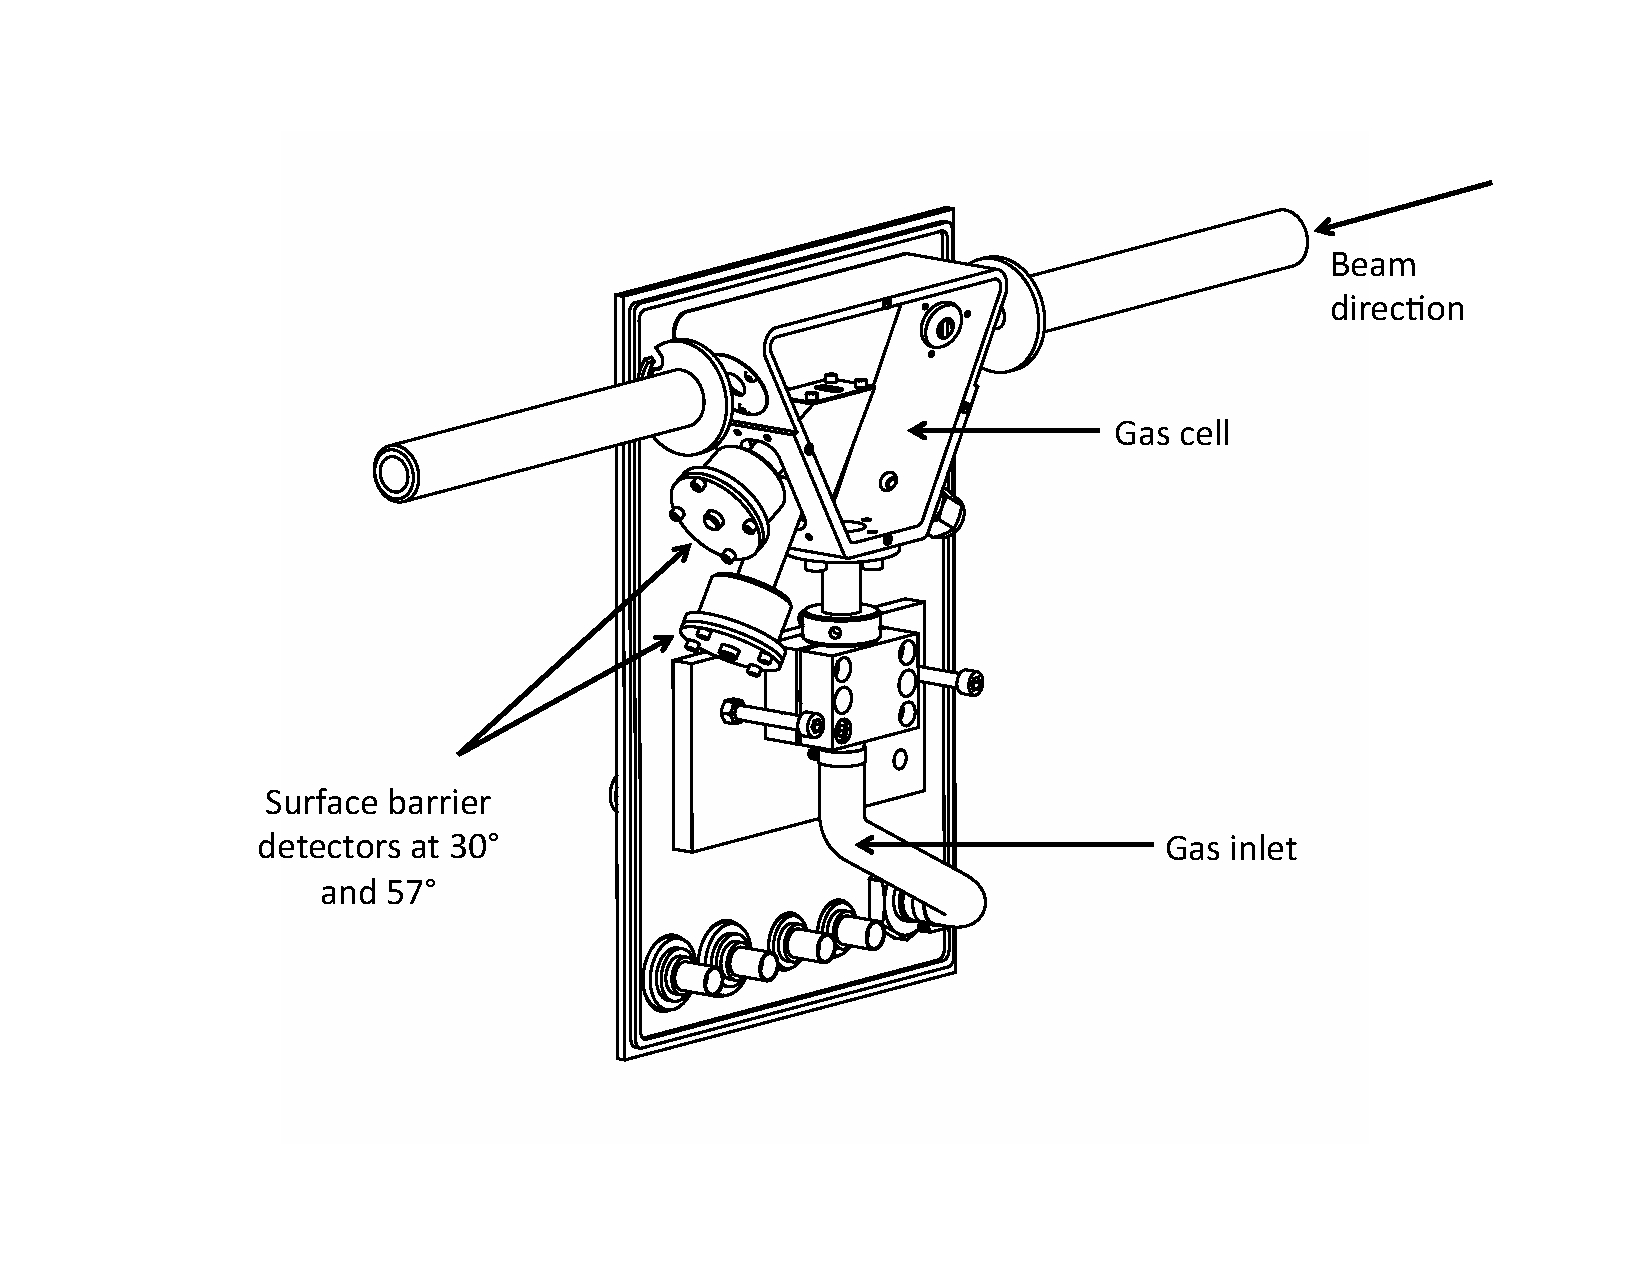
\includegraphics{dra_gas_target}
}
%\vspace{5cm}       % Give the correct figure height in cm
\caption{The DRAGON windowless gas target, showing the trapezoidal gas volume and gas inlet, surface barrier detectors and inner pumping tubes.  }
\label{fig:dra_gas_target}
\end{figure}

The ion optical configuration of DRAGON is a {\bf MEME} design, consisting of magnetic and electric  dipole elements of bending angles $\phi=$50$^{\circ}$,20$^{\circ}$,75$^{\circ}$ and 35$^{\circ}$, and bending radii $\rho$=100 cm, 200 cm, 81.3 cm and 250 cm respectively (figure \ref{fig:dra_optics}). The particular configuration was designed specifically around the recoil distribution expected from the $^{15}$O($\alpha ,\gamma$)$^{19}$Ne reaction at $E_{c.m.}=0.51$ MeV. It was thus designed with a geometric acceptance of $\pm21$ mrad at the central energy, and an energy acceptance of $\pm4\%$ at the central trajectory. 
\begin{figure*}
\begin{center}
\resizebox{1.6\columnwidth}{!}{
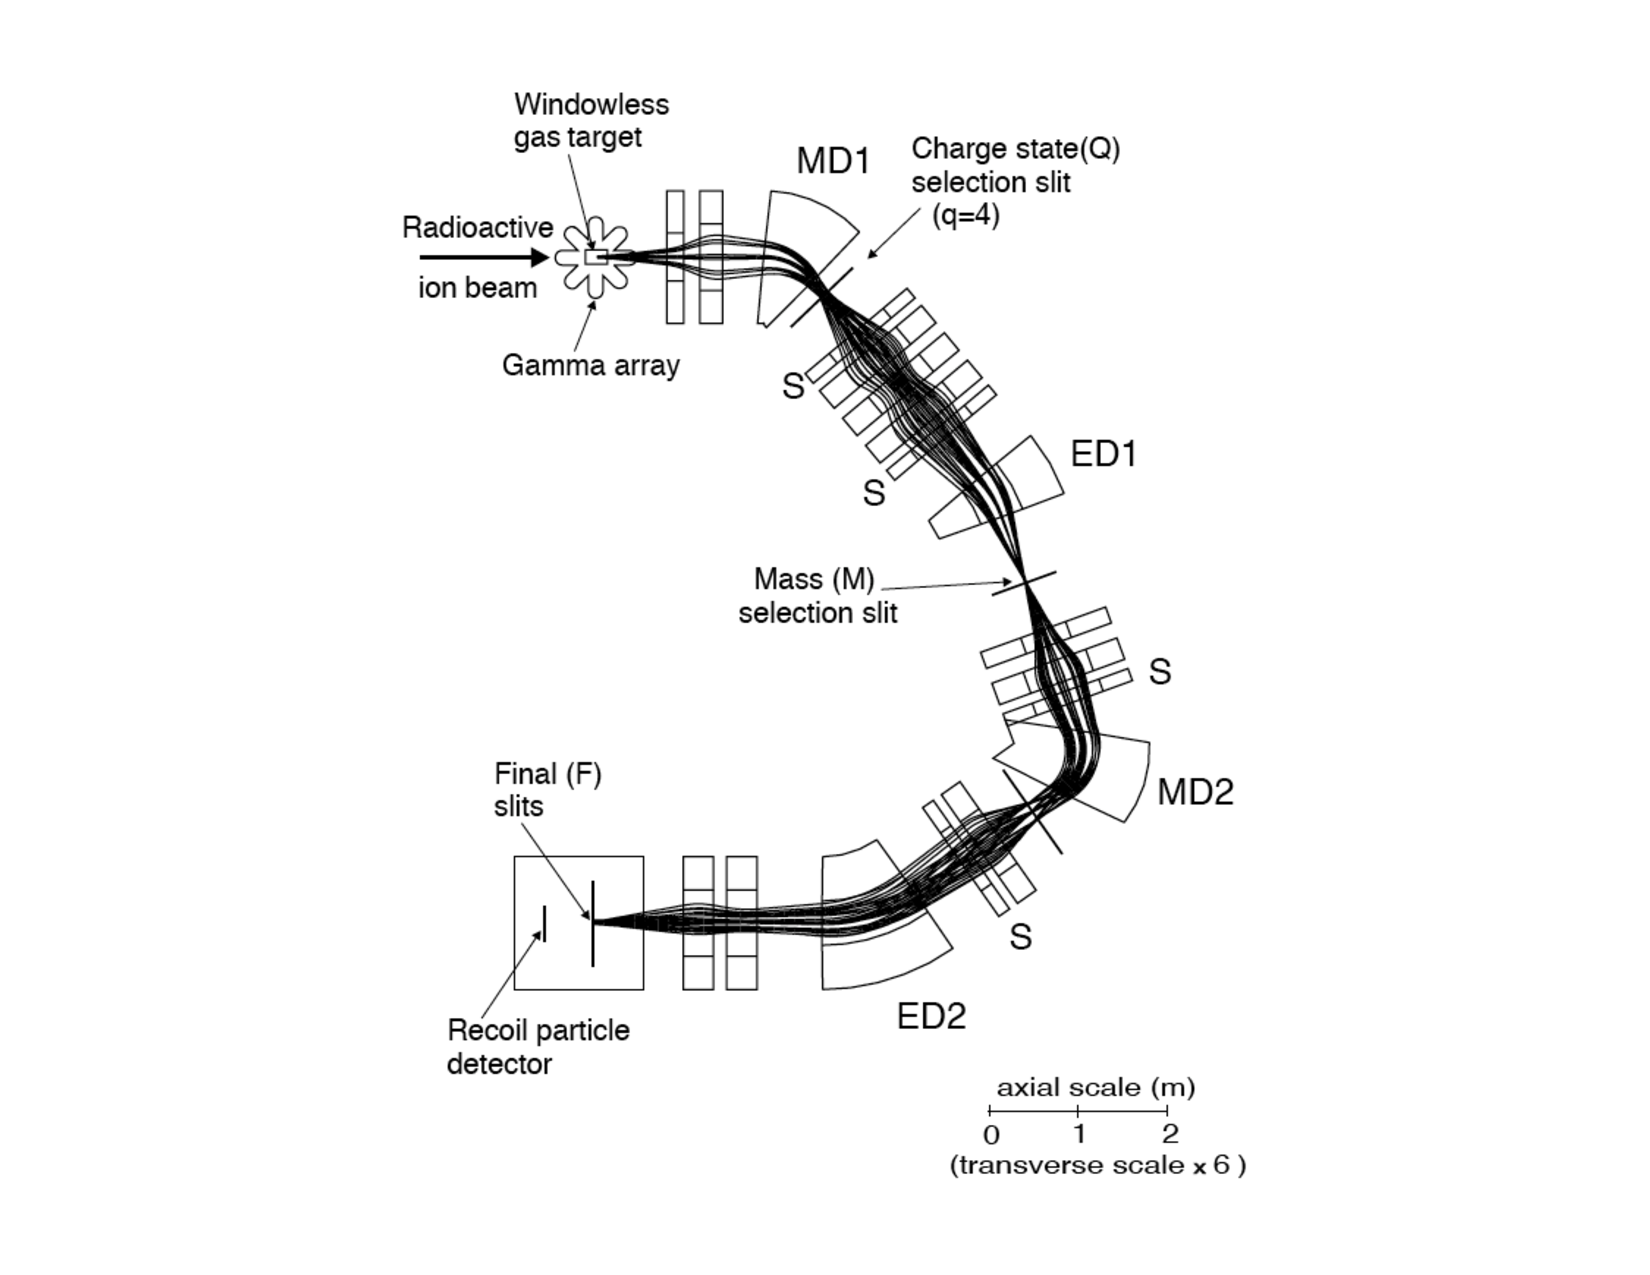
\includegraphics{dra_optics}
}
%\vspace{5cm}       % Give the correct figure height in cm
\caption{Schematic representation of the DRAGON recoil separator (taken from \cite{hut03}). The electrostatic dipoles, with respective lengths 0.7 and 1.57~m and voltages $\pm$200 and $\pm$160~kV, give a proxy figure of merit 780~kV$\cdot$m.  Design angular acceptance was 2$\times$21~mrad with beam energies in the range 0.15 to 1.5~MeV per nucleon. The transverse scale has been magnified 6X to display apertures and trajectories.}
\label{fig:dra_optics}
\end{center}
\end{figure*}

The first magnetic dipole (MD1) of the separator is used to select a single charge state for beam and recoils, using a set of slits located at the first energy-dispersed focus after MD1. This focus has an energy dispersion of 0.3 cm/\% and a magnification of -0.44 in the horizontal direction. The energy of the beam/recoils in their chosen charge state can thus be measured by centring on the slits at this focus and relating the magnetic field - measured using an NMR probe positioned in the central flat field region of the dipole - to the beam energy via the magnet calibration constant, which has been determined using several well-known stable beam proton capture resonances. Thus a direct measurement of the beam energy with and without gas in the target allows a determination of the target energy loss, which when combined with the effective length, gives the stopping power. 

The first mass-separation stage stage of the DRAGON separator occurs after the first electric dipole element, at a set of slits at the mass-dispersed achromatic focus. The second stage of the separator is essentially a copy of the first. The overall mass resolution at the final focus of the separator is around 0.3\% for a typical object size at the gas target central position.  

%Acceptance, suppression, rigidity, background rejection, resonance energy determination (both BGOs)
The overarching quality of DRAGON is the separator beam suppression. As can be seen in ref. \cite{hutc08}, the raw beam suppression of the separator (for proton capture)\footnote{In general, for alpha-capture reactions on a given beam mass, better beam suppression is achieved. This can be compounded further in a few light-mass cases where the availability of beam charge-states is reduced, as can be seen in the extreme case of $^{3}$He($\alpha$,$\gamma$)$^{7}$Be, where a $^{7}$Be charge state can be selected for which there is no similar beam A/Q, leading to extremely high separator suppression values (see ref. \cite{sju12}).} is on the order of 10$^{8}$-10$^{13}$, depending on the incident beam energy. This is directly correlated to the emittance of the delivered beam, which results in a larger and more divergent beam at the target position for lower energies, and thus frame scattering in the target and pumping tube region, and elsewhere in the separator, can result in orders of magnitude difference in the fraction of incident beam particles that reach the final focus. As it stands, this is well suited to the range of radiative capture reactions to be studied, with reaction yields on the order of down to 10$^{-14}$ reaction per incident beam particle. This means that for weak reactions, the 'leaky beam' rate at the focal plane detectors can be a couple to a few orders of magnitude lower or higher than the expected reaction signal. Local time of flight and particle energy or stopping power measurement can then be used to identify the particles, leading to higher effective orders of background suppression. In DRAGON's case a 5 cm $\times$ 5 cm, 256-quasi-pixel double-sided silicon strip detector can be used, or a 4-anode isobutane-filled ionization chamber, for final particle detection, the latter offering an additional degree of atomic-number discrimination through differential energy loss of the ions through the anode regions. These detectors are located approximately 60 cm from DRAGON's focal plane.

On either side of the focal plane, separated by 50 cm are two microchannel plates offering a minimally-destructive local time-of-flight system capable of ~400 ps resolution, sufficient to provide excellent mass separation between the reaction products and leaky beam particles. Ref. \cite{vock09} provides a detailed description of this device, which relies on thin diamond-like-carbon (DLC) foils and electroformed meshes to function according to requirements. 

The DRAGON separator is designed for beam rigidities of up to 0.55 T$\cdot$m. The limiting factors are (a) the maximum achievable magnetic field strength at the first magnetic dipole and (b) the maximum sustainable electric voltage between the electrodes of the first electric dipole. The magnetic field limit is the limiting factor below ion energies of $1.34A$ MeV, for a maximum field of 0.55 T, while the electric field is the limit above this energy, corresponding to a maximum setpoint voltage of 230 kV (corresponding to a field strength of 4.6 MV/m). Figure \ref{fig:rigidity} shows the limiting curves for maximum bendable ion energy versus ion mass-to-charge ratio.   

\begin{figure}\resizebox{1.0\columnwidth}{!}{
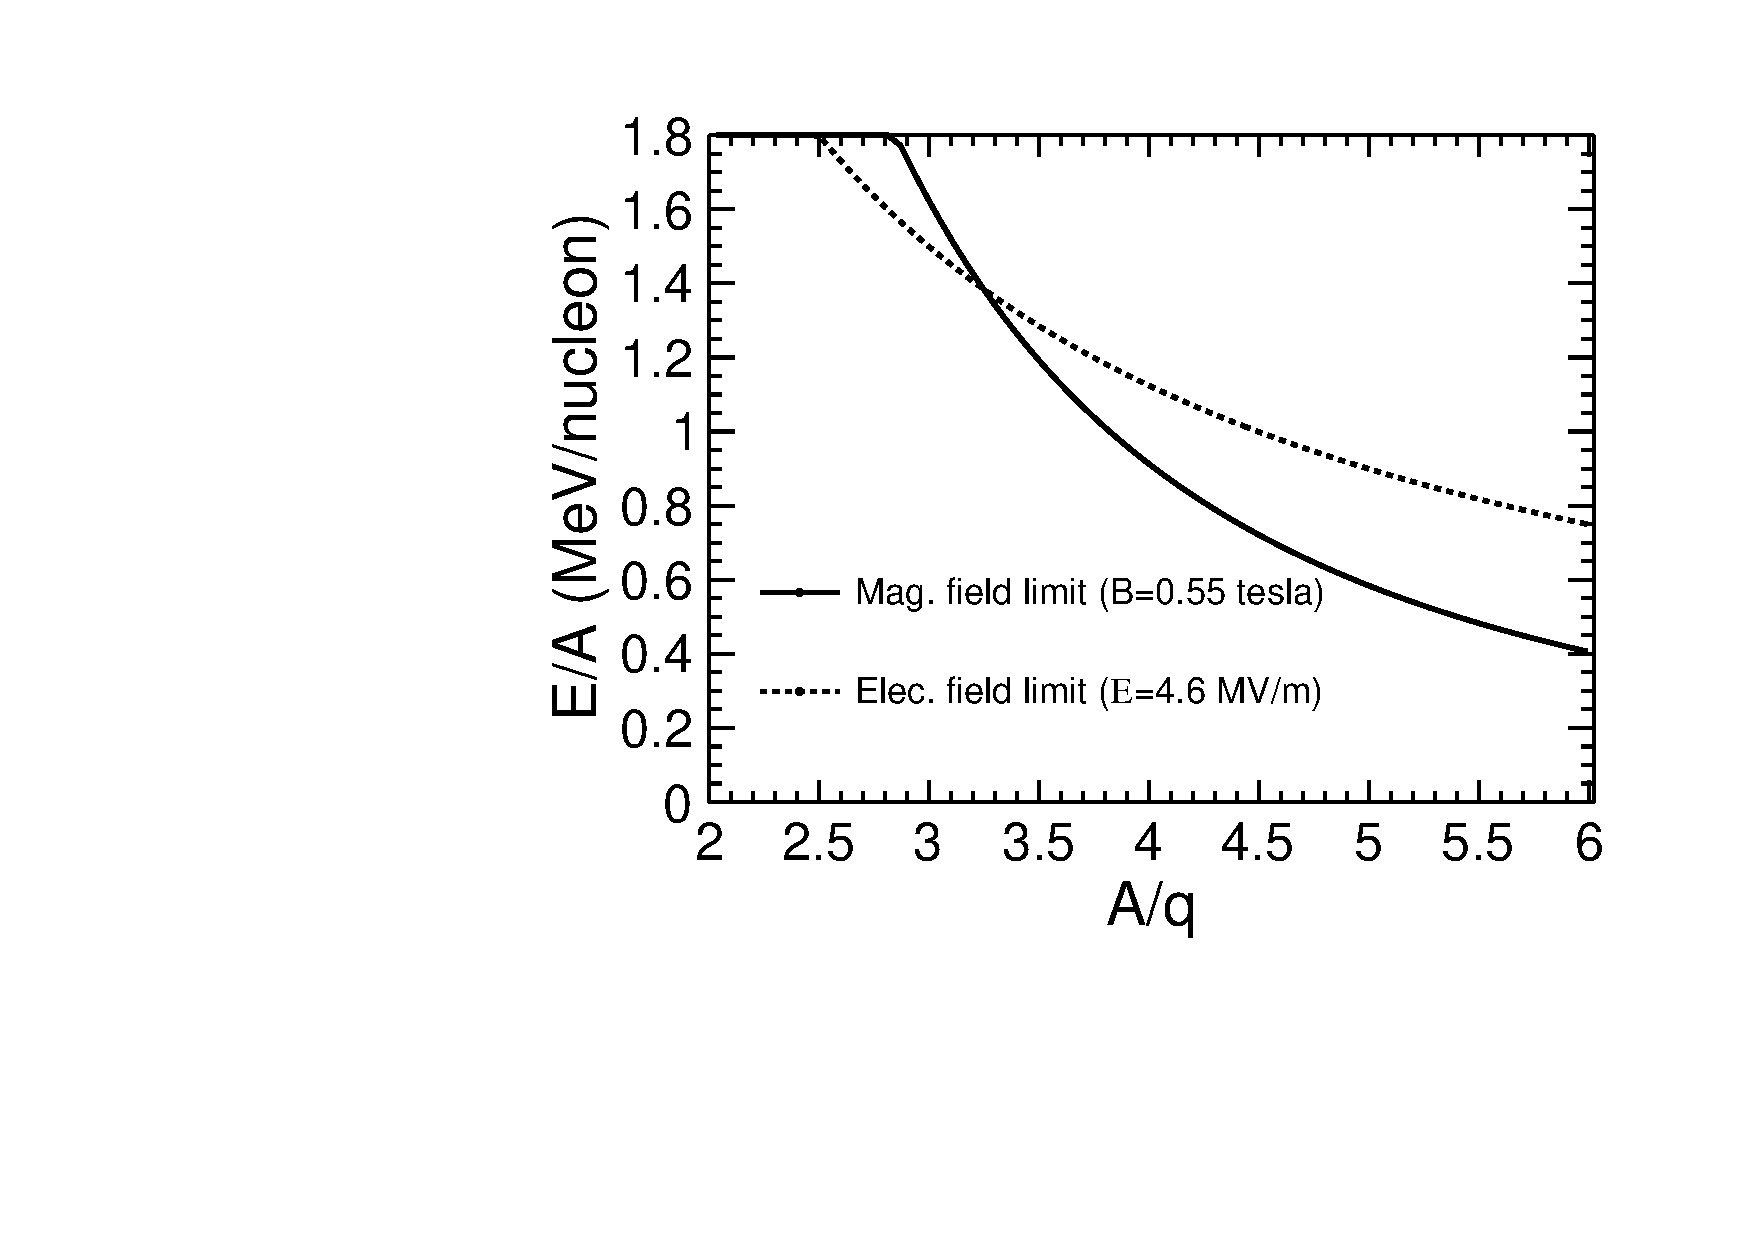
\includegraphics{rigidity}
}
%\vspace{5cm}       % Give the correct figure height in cm
\caption{Magnetic and electric limits for the DRAGON separator, showing the maximum ion energy that can be bent around the magnetic and electric dipoles for a given mass-to-charge ratio. Above $1.38A$ MeV, the limit is the sustainable field on the electric dipole. Below this, the power supply and cooling on the magnetic dipole is the hardware limit.}
\label{fig:rigidity}
\end{figure}

To provide additional background rejection to the focal plane detectors, recoil ions are tagged with prompt $\gamma$-rays emitted from the reaction at the gas target. These are detected using a 30-element bismuth germanate (BGO) array consisting of hexagonal crystals roughly 6~cm in diameter and 8~cm deep arranged so as to give nearly 4$\pi$ solid angle coverage \cite{gig03}. BGO was chosen primarily because of its high efficiency (high absorption for $\gamma$-rays due to the high material density and a large scintillation light output), but also because of its relatively inexpensive nature compared to faster or brighter scintillators such as lanthanum bromide (LaBr$_{3}$) or lutetium oxyorthosilicate (LSO). Because the recoil ions are the primary detection object, high energy resolution is not really necessary, the 10\% or so given by BGO being sufficient for most purposes. The segmentation of the array also allows individual cascade $\gamma$ rays to be detected, giving an overall very high efficiency in the range 40-80\% dependent on the energies and quantity of $\gamma$ rays\footnote{In a given cascade of $N$ $\gamma$ rays, the probability of detecting at least one of them is given by $P=1-\Pi^{N}_{i=1}(1-\epsilon_{i})$ where $\epsilon_i$ here represents the efficiency of detecting the $i$th $\gamma$ ray and encompasses all geometric and energy-dependent factors. With typical values of $\epsilon$ around the 40\% mark for the almost $4\pi$ coverage DRAGON BGO array, it is easy to see how cascades of 3 $\gamma$ rays for example, can lead to high detection efficiency.}. 

By detecting prompt $\gamma$ rays, and by determining the time-of-flight between them and the recoil ion detection, 2-3 orders of magnitude further effective beam suppression (random background rejection) can be achieved on top of the raw separator suppression and particle identification. The BGO efficiency (see ref. \cite{gig03} for details on how it is measured) however, is the major systematic error in such a measurement, and it dominates the total systematic error of the experiment.  

The BGO array, because of its segmentation along the beam (z) axis, can also provide information on the location of the reaction origin for a narrow resonance via the BGO hit pattern. This, coupled with the beam-in-gas stopping power (derived by measuring the beam energy at the energy-dispersed focus with and without gas in the target) allows a determination of the resonance energy, to a precision of 0.5\% \cite{hut12}.
 
The DRAGON facility started its experimental program by extensively studying the radioactive beam reaction $^{21}$Na($p,\gamma$)$^{22}$Mg during 2000-2003 \cite{dau04}, following over the years with the other RIB studies  $^{26g}$Al($p,\gamma$)$^{27}$Si \cite{rui06}, $^{23}$Mg($p,\gamma$)$^{24}$Al \cite{eri10} and $^{18}$F($p,\gamma$)$^{19}$Ne \cite{ake13} (some of these are discussed in more detail in the following sections). At the time of writing of this article DRAGON had recently performed measurements of $^{26m}$Al($p,\gamma$)$^{27}$Si. In addition studies have been performed for the stable beam alpha-capture reactions $^{12}$C($\alpha$,$\gamma$)$^{16}$O \cite{mat06}, $^{40}$Ca($\alpha$,$\gamma$)$^{44}$Ti \cite{voc07,voc08}, $^{17}$O($\alpha$,$\gamma$)$^{21}$Ne, $^{16}$O($\alpha$,$\gamma$)$^{20}$Ne \cite{hag12b} and $^{3}$He($\alpha$,$\gamma$)$^{7}$Be \cite{sin12}, and for the proton-capture reactions ~~~$^{17}$O($p,\gamma$)$^{18}$F \cite{hag12} and $^{33}$S($p,\gamma$)$^{34}$Cl \cite{fal13}. In addition, a high mass capture reaction study was performed at DRAGON to demonstrate its ability to perform as a recoil separator far beyond its design limit. The reaction chosen was $^{58}$Ni($p,\gamma$)$^{59}$Cr \cite{Sim13}, and the success of this study prompted the consideration of more alpha capture reactions above the $A=76$ region for the p-process.  Forays into this region began at DRAGON in earnest with the measurement of $^{76}$Se($\alpha$,$\gamma$)$^{80}$Kr \cite{Fal14}. 




 
